%% LaTeX source of Chapter 5 of the thesis.
%% NEVER compile this file. Complie 'thesis.tex' instead.

\chapter{结果分析}
\label{Chapter 5}

我们通过第三章给出的核心算法,以及第四章的需求和设计,来对时序数据压缩的情况进行模拟与分析。

\section{示例说明}
\label{5.1}
通过第四章的描述我们知道,压缩模拟的过程中,我们先通过模拟时序数据发生器,来生成时序数据,原始数据的产生时间间隔为10ms,当原始数据生成以后我们对每一个区间按照区间分隔算法来进行数据区间的分割,当区间分割完毕之后,我们通过数据区间的合并算法对那些数据点过密也就是区间内的数据点数超过限制的区间进行合并,然后我们通过数据生成算法来生成压缩后的数据。最后我们可以通过基于浏览器来显示我们的可视化数据。

\section{模拟过程}
\label{5.2}

\subsection{时序数据模拟产生}
\label{5.21}
在程序的实际实现过程中,数据的维数接近100,此处由于篇幅限制,我们将维数降低以使结果更加明显,程序运行的过程如图所示,\ref{Figure 5-1-1}此处我们将输出数据重定向到了活动窗口。

\begin{figure}[h!]
	\centering
	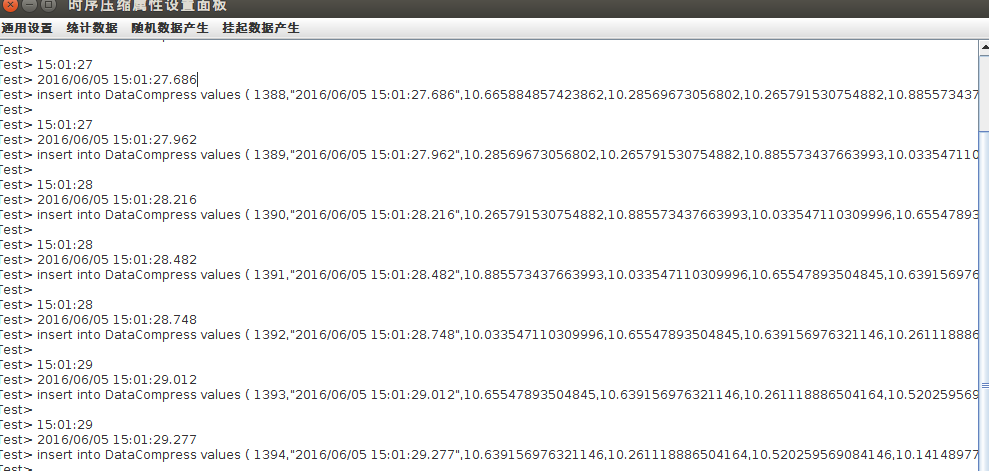
\includegraphics[scale=0.35]{./images/figure-5-1}
	\caption{模拟时序数据发生器}
	\label{Figure 5-1-1}
\end{figure}



如图对应的原始表如下:

\begin{center}
  \begin{tabular}{ | p{1.5cm} | p{1.5cm} | p{1.5cm} | p{1.5cm} | p{1.5cm} | p{1.5cm}|p{1.5cm}}
    \hline
    T  & D$_{1}$ & D$_{2}$ & D$_{3}$ & D$_{4}$  & D$_{5}$ &  D$_{6}$  \\ \hline
    1  & 10.6     & 10.2     & 10.2     & 10.8  &10.8     &   10.8     \\ \hline
    2  &10.2      &10.2      &10.8      &10.0   &10.0     &   10.0     \\  \hline
    3  &10.2      &10.2      &10.8      &10.0   &10.0     &   10.0      \\ \hline
    4 &10.8      &10.0      &10.0      &10.1    &10.0     &   10.0   \\ \hline
    5 &10.8      &10.0      &10.0      &10.1    &10.1     &   10.2    \\ \hline
    6 &10.7      &10.2      &10.2      &10.2    &10.0     &   10.2    \\ \hline
    7 &10.9      &10.2      &10.3      &10.2    &10.3     &   11.0     \\ \hline
    \hline
  \end{tabular}
\end{center}


\subsection{时序数据区间分隔}
\label{5.22}
通过原始数据的每一列我们进行区间划分,划分的规则如下:

\begin{lstlisting}
D1  [1,1]  [2,3]  [4,7]
D2  [1,7]
D3  [1,1]  [2,3]  [4,7]
D4  [1,1]  [2,7]
D5  [1,1]  [2,7]  
D6  [1,1]  [2,7]
\end{lstlisting}


\subsection{区间合并与数据生成}
\label{5.23}
由时序数据区间分隔算法产生的区间点包括[1,1],[2,3],[4,7],由这些时间点的生成的区间如下表所示:

\begin{center}
  \begin{tabular}{ | p{1.5cm} | p{1.5cm} | p{1.5cm} | p{1.5cm} | p{1.5cm} | p{1.5cm}|p{1.5cm}}
    \hline
    T  & D$_{1}$ & D$_{2}$ & D$_{3}$ & D$_{4}$  & D$_{5}$ &  D$_{6}$  \\ \hline
    1  & 10.6     & 10.2     & 10.2     & 10.8  &10.8     &   10.8     \\ \hline
    2  &10.2      &10.2      &10.8      &10.0   &10.0     &   10.0     \\  \hline
    3  &10.8      &10.1      &10.8      &10.1   &10.1     &   10.1      \\ \hline
    \hline
  \end{tabular}
\end{center}

\newpage 

\subsection{可视化示例}
\label{5.24}
时序数据通过可视化后的显示如下\ref{Figure 5-1-2},从图中我们可以观察到统计数据的开始值,结束值,最大值,最小值,以及分布情况。

\begin{figure}[h!]
	\centering
	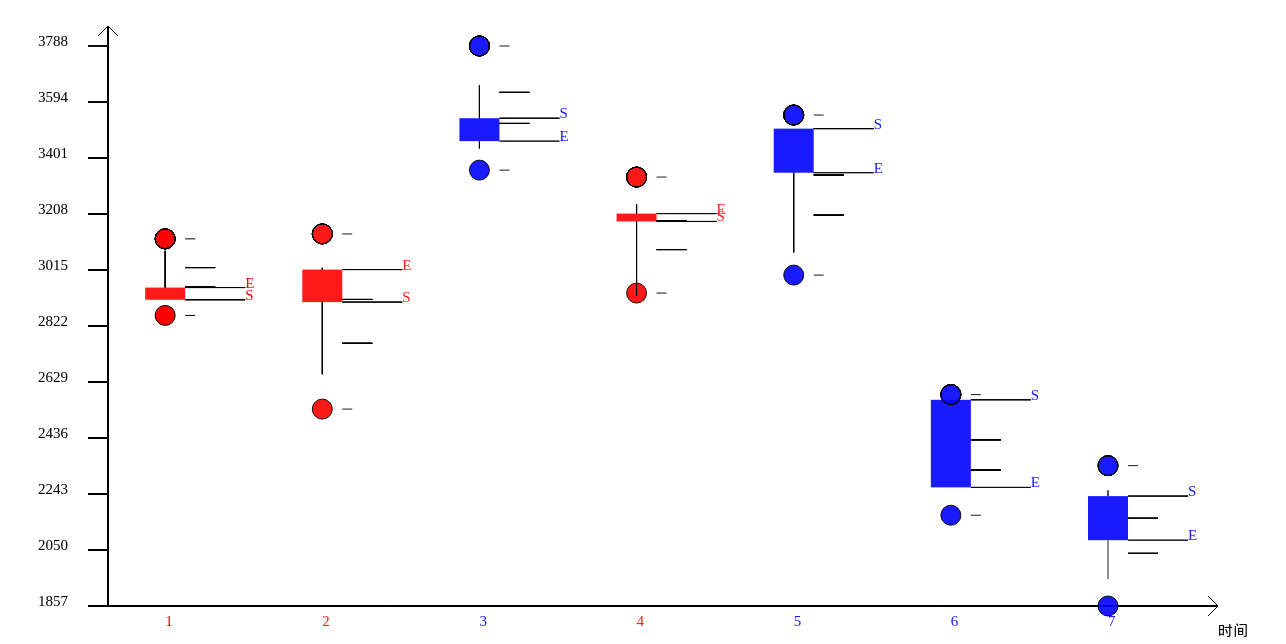
\includegraphics[scale=0.35]{./images/figure-5-2}
	\caption{模拟时序数据发生器}
	\label{Figure 5-1-2}
\end{figure}

图中包含以下有效信息:

\begin{enumerate}[(1)]
	\item 红颜色方块代表开始值大于结束值,蓝色方块为开始值小于结束值。
	\item 开始值和结束值被实体方块包围。
	\item 次短线代表3/4位数,和1/4位数。
	\item 最短线代表最大值和最小值。
\end{enumerate}





\subsection{压缩结果分析}
\label{5.25}
通过上述的过程我们可以看出,原始数据的时间点数为6,而压缩处理过后产生的时间点数为3,这在存储的过程
中减少了一半的存储量,这是在我们的波动误差约为0.5所得出的结论,如果我们的误差设置为1,那么压缩效果
可以达到1/6,由此可见,在条件允许的情况下,这能节省大量的存储空间。










